\chapter{Lista}

\index{lista}

\emph{Lista} (\emph{list}) on taulukkoa muistuttava tietorakenne,
joka sisältää joukon alkioita,
jotka ovat peräkkäin tietyssä järjestyksessä.
Esimerkiksi $[3,7,2,5]$ on lista, joka sisältää neljä alkiota.
Haluamme toteuttaa listan niin,
että pääsemme käsiksi listalla olevaan alkioon
sen kohdan perusteella
ja lisäksi pystymme lisäämään ja poistamaan alkioita.

Tässä luvussa tutustumme kahteen lähestymistapaan listan luomiseen.
Ensin toteutamme taulukkolistan,
jossa listan alkiot tallennetaan taulukkoon.
Tämän jälkeen toteutamme linkitetyn listan,
joka muodostuu toisiinsa viittaavista solmuista.
Kuten tulemme huomaamaan, molemmissa listan toteutuksissa on omat
hyvät ja huonot puolensa.

\section{Taulukkolista}

\index{taulukkolista}

\emph{Taulukkolista} (\emph{array list}) on lista, joka on tallennettu taulukkona.
Koska taulukon alkiot sijaitsevat aina peräkkäin muistissa,
pääsemme käsiksi mihin tahansa listan alkioon ajassa $O(1)$.
Haasteena toteutuksessa on kuitenkin,
että taulukon koko on \emph{kiinteä} ja jos haluamme
muuttaa listan kokoa, meidän täytyy varata uusi taulukko
ja kopioida sinne vanhan taulukon sisältö.

\subsection{Muutokset lopussa}

Toteutamme ensin taulukkolistan, jossa alkioiden
lisäykset ja poistot tapahtuvat listan lopussa.
Tallennamme listan taulukkona niin,
että tietty määrä alkioita taulukon alussa on listan käytössä
ja loput tyhjät kohdat on varattu tuleville alkioille.
Tämän ansiosta pystymme lisäämään uuden alkion listalle
ajassa $O(1)$, jos taulukossa on tilaa,
koska meidän riittää vain ottaa käyttöön seuraava
vapaana oleva kohta taulukosta.

Kuva \ref{fig:listau} näyttää esimerkin,
jossa taulukossa on tilaa yhteensä kahdeksalle alkiolle
ja siihen on tallennettu lista $[3,7,2,5]$.
Taulukon neljä ensimmäistä kohtaa ovat siis listan käytössä
ja muut ovat varalla tulevia alkioita varten.
Kun lisäämme listan loppuun uuden alkion 6,
otamme käyttöön taulukosta uuden kohdan, johon alkio sijoitetaan.

\begin{figure}
\center
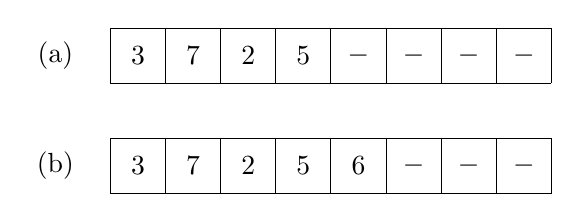
\begin{tikzpicture}[scale=0.7]
\begin{scope}
\draw (0,0) grid (8,1);
\node at (-1,0.5) {(a)};
\node at (0.5,0.5) {$3$};
\node at (1.5,0.5) {$7$};
\node at (2.5,0.5) {$2$};
\node at (3.5,0.5) {$5$};
\node at (4.5,0.5) {$-$};
\node at (5.5,0.5) {$-$};
\node at (6.5,0.5) {$-$};
\node at (7.5,0.5) {$-$};
\end{scope}
\begin{scope}[yshift=-2cm]
\draw (0,0) grid (8,1);
\node at (-1,0.5) {(b)};
\node at (0.5,0.5) {$3$};
\node at (1.5,0.5) {$7$};
\node at (2.5,0.5) {$2$};
\node at (3.5,0.5) {$5$};
\node at (4.5,0.5) {$6$};
\node at (5.5,0.5) {$-$};
\node at (6.5,0.5) {$-$};
\node at (7.5,0.5) {$-$};
\end{scope}
\end{tikzpicture}
\caption{(a) Lista $[3,7,2,5]$ tallennettuna taulukkoon. (b) Listan loppuun lisätään alkio 6.}
\label{fig:listau}
\end{figure}

\begin{figure}
\center
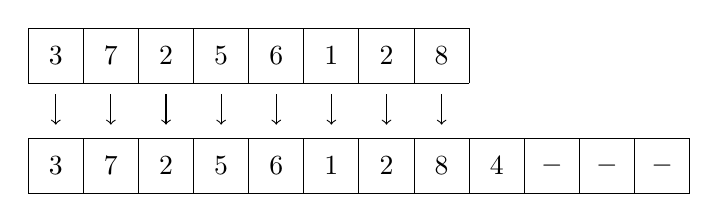
\begin{tikzpicture}[scale=0.7]
\begin{scope}
\draw (0,0) grid (8,1);
\node at (0.5,0.5) {$3$};
\node at (1.5,0.5) {$7$};
\node at (2.5,0.5) {$2$};
\node at (3.5,0.5) {$5$};
\node at (4.5,0.5) {$6$};
\node at (5.5,0.5) {$1$};
\node at (6.5,0.5) {$2$};
\node at (7.5,0.5) {$8$};
\foreach \x in {0,...,7} \draw[->] (\x+0.5,-0.2) -- (\x+0.5,-0.75);
\end{scope}
\begin{scope}[yshift=-2cm]
\draw (0,0) grid (12,1);
\node at (0.5,0.5) {$3$};
\node at (1.5,0.5) {$7$};
\node at (2.5,0.5) {$2$};
\node at (3.5,0.5) {$5$};
\node at (4.5,0.5) {$6$};
\node at (5.5,0.5) {$1$};
\node at (6.5,0.5) {$2$};
\node at (7.5,0.5) {$8$};
\node at (8.5,0.5) {$4$};
\node at (9.5,0.5) {$-$};
\node at (10.5,0.5) {$-$};
\node at (11.5,0.5) {$-$};
\end{scope}
\end{tikzpicture}
\caption{Taulukkoon ei mahdu enää uutta alkiota. Meidän täytyy varata uusi suurempi taulukko
ja kopioida vanhan taulukon sisältö sinne.}
\label{fig:lisuus}
\end{figure}

Mitä tapahtuu sitten, kun jossain vaiheessa koko taulukko
on täynnä eikä uusi listalle lisättävä alkio mahdu enää taulukkoon?
Tällöin meidän täytyy ensin varata uusi suurempi taulukko ja
kopioida kaikki vanhan taulukon alkiot siihen.
Vasta tämän jälkeen voimme lisätä uuden alkion listalle.
Tämä vie aikaa $O(n)$, koska kopioimme kaikki listan alkiot
uuteen paikkaan muistissa.
Esimerkiksi kuvassa \ref{fig:lisuus} uusi alkio 4 ei mahdu taulukkoon,
joten joudumme varaamaan uuden taulukon ja kopioimaan alkiot.

Olemme saaneet siis aikaan listan, jossa lisääminen
vie aikaa \emph{joko} $O(1)$ tai $O(n)$ riippuen siitä,
mahtuuko alkio nykyiseen taulukkoon vai täytyykö
meidän varata uusi taulukko.
Jotta lista olisi käyttökelpoinen, hidas $O(n)$-operaatio
ei saisi esiintyä liian usein.
Osoittautuu, että saavutamme tämän tavoitteen,
kunhan varaamme uuden taulukon aina reilusti aiempaa suuremmaksi.
Tavanomainen ratkaisu on \emph{kaksinkertaistaa} taulukon koko aina,
kun varaamme uuden taulukon.
Kun toimimme näin, jokaisen alkion lisääminen listalle vie
\emph{keskimäärin} vain $O(1)$ aikaa.

Miksi aikaa kuluu keskimäärin vain $O(1)$?
Tarkastellaan tilannetta, jossa listaan lisätään alkioita
ja taulukkoa kasvatetaan viimeisen kerran,
kun listassa on $n$ alkiota.
Haluamme arvioida, montako alkiota kopioidaan
taulukosta toiseen prosessin aikana.
Koska taulukon koko kaksinkertaistuu joka vaiheessa,
kopioinnista tuleva lisäkustannus on
$n+n/2+n/4+n/8+\dots = O(n)$,
eli keskimääräinen kustannus alkiota kohden on $O(1)$.
Taulukon kasvattamisen vaikutus kokonaisuuteen
on siis pieni.

\begin{figure}
\center
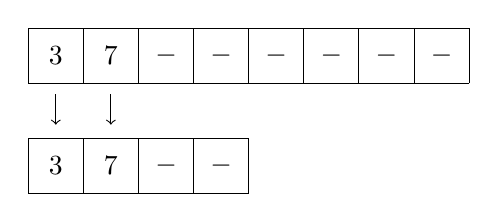
\begin{tikzpicture}[scale=0.7]
\begin{scope}
\draw (0,0) grid (8,1);
\node at (0.5,0.5) {$3$};
\node at (1.5,0.5) {$7$};
\node at (2.5,0.5) {$-$};
\node at (3.5,0.5) {$-$};
\node at (4.5,0.5) {$-$};
\node at (5.5,0.5) {$-$};
\node at (6.5,0.5) {$-$};
\node at (7.5,0.5) {$-$};
\foreach \x in {0,...,1} \draw[->] (\x+0.5,-0.2) -- (\x+0.5,-0.75);
\end{scope}
\begin{scope}[yshift=-2cm]
\draw (0,0) grid (4,1);
\node at (0.5,0.5) {$3$};
\node at (1.5,0.5) {$7$};
\node at (2.5,0.5) {$-$};
\node at (3.5,0.5) {$-$};
\end{scope}
\end{tikzpicture}
\caption{Poistojen jälkeen taulukon koko on käynyt tarpeettoman suureksi,
ja puolitamme taulukon koon.}                                                                        
\label{fig:lispoi}
\end{figure}

Voimme poistaa alkion listan lopusta aina $O(1)$-ajassa,
koska taulukon kokoa ei tarvitse koskaan suurentaa.
Tässä voi kuitenkin tulla ongelmaksi, että monien poistojen
jälkeen taulukossa on turhan paljon tyhjää tilaa lopussa.
Voimme soveltaa tässä käänteisesti samaa ideaa kuin lisäämisessä:
jos poistamisen jälkeen vain \emph{neljännes} taulukosta on käytössä,
puolitamme taulukon koon.
Kuva \ref{fig:lispoi} näyttää esimerkin tällaisesta tilanteesta.
Tällä tavalla myös poistamiset vievät keskimäärin aikaa $O(1)$.

Miksi emme voisi varata heti aluksi niin suurta taulukkoa,
että lopullinen lista mahtuisi siihen varmasti?
Tässä olisi huonona puolena, että listamme tuhlaisi paljon muistia.
Algoritmissa saattaa olla samaan aikaan käytössä monia listoja,
ja haluamme, että listalle varattu taulukko on samaa kokoluokkaa
kuin listan todellinen sisältö.

\subsection{Muutokset alussa ja lopussa}

Melko samaan tapaan voimme myös luoda taulukkolistan,
joka sallii tehokkaat alkioiden lisäykset ja poistot
sekä listan alussa että lopussa.
Jotta tämä onnistuisi, muutamme listan tallennustapaa niin,
että lista voi alkaa ja päättyä missä tahansa taulukon
kohdassa ja listan sisältö voi tarvittaessa jatkua taulukon lopusta alkuun.

\begin{figure}
\center
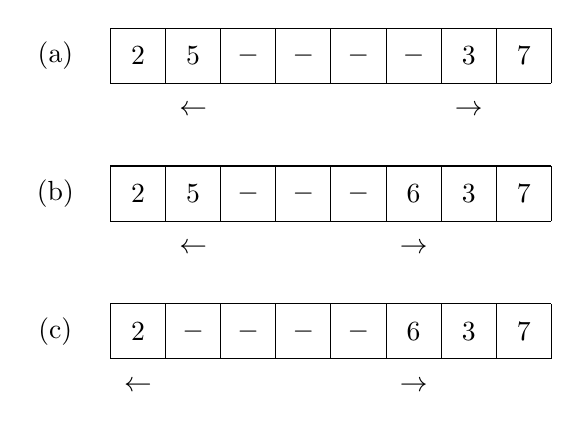
\begin{tikzpicture}[scale=0.7]
\begin{scope}
\draw (0,0) grid (8,1);
\node at (-1,0.5) {(a)};
\node at (0.5,0.5) {$2$};
\node at (1.5,0.5) {$5$};
\node at (2.5,0.5) {$-$};
\node at (3.5,0.5) {$-$};
\node at (4.5,0.5) {$-$};
\node at (5.5,0.5) {$-$};
\node at (6.5,0.5) {$3$};
\node at (7.5,0.5) {$7$};
\node at (1.5,-0.5) {$\leftarrow$};
\node at (6.5,-0.5) {$\rightarrow$};
\end{scope}
\begin{scope}[yshift=-2.5cm]
\draw (0,0) grid (8,1);
\node at (-1,0.5) {(b)};
\node at (0.5,0.5) {$2$};
\node at (1.5,0.5) {$5$};
\node at (2.5,0.5) {$-$};
\node at (3.5,0.5) {$-$};
\node at (4.5,0.5) {$-$};
\node at (5.5,0.5) {$6$};
\node at (6.5,0.5) {$3$};
\node at (7.5,0.5) {$7$};
\node at (1.5,-0.5) {$\leftarrow$};
\node at (5.5,-0.5) {$\rightarrow$};
\end{scope}
\begin{scope}[yshift=-5cm]
\draw (0,0) grid (8,1);
\node at (-1,0.5) {(c)};
\node at (0.5,0.5) {$2$};
\node at (1.5,0.5) {$-$};
\node at (2.5,0.5) {$-$};
\node at (3.5,0.5) {$-$};
\node at (4.5,0.5) {$-$};
\node at (5.5,0.5) {$6$};
\node at (6.5,0.5) {$3$};
\node at (7.5,0.5) {$7$};
\node at (0.5,-0.5) {$\leftarrow$};
\node at (5.5,-0.5) {$\rightarrow$};
\end{scope}
\end{tikzpicture}
\caption{(a) Lista $[3,7,2,5]$ tallennettuna taulukkoon.
(b) Listan alkuun lisätään alkio 6.
(c) Listan lopusta poistetaan alkio 5.}
\label{fig:lismol}
\end{figure}


\begin{figure}
\center
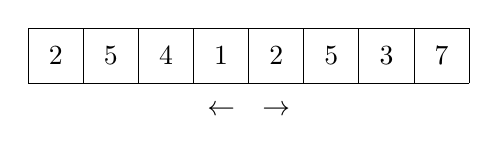
\begin{tikzpicture}[scale=0.7]
\begin{scope}
\draw (0,0) grid (8,1);
\node at (0.5,0.5) {$2$};
\node at (1.5,0.5) {$5$};
\node at (2.5,0.5) {$4$};
\node at (3.5,0.5) {$1$};
\node at (4.5,0.5) {$2$};
\node at (5.5,0.5) {$5$};
\node at (6.5,0.5) {$3$};
\node at (7.5,0.5) {$7$};
\node at (3.5,-0.5) {$\leftarrow$};
\node at (4.5,-0.5) {$\rightarrow$};
\end{scope}
\end{tikzpicture}
\caption{Lista täyttää koko taulukon, emmekä voi lisätä uutta alkiota.
Ratkaisuna on varata listalle uusi suurempi taulukko.}
\label{fig:lismol2}
\end{figure}

Kuva \ref{fig:lismol} näyttää esimerkin listan $[3,7,2,5]$
uudesta tallennustavasta.
Merkki $\rightarrow$ osoittaa kohdan, josta lista alkaa,
ja merkki $\leftarrow$ osoittaa kohdan, johon lista päättyy.
Kun haluamme lisätä alkion listan alkuun,
siirrymme vasemmalle kohdasta $\rightarrow$,
ja kun haluamme lisätä alkion listan loppuun,
siirrymme oikealle kohdasta $\leftarrow$.
Kun haluamme poistaa alkioita listasta,
menettelemme käänteisesti.

Jos kohdat $\rightarrow$ ja $\leftarrow$ ovat vierekkäin,
taulukko on täynnä, emmekä voi enää lisätä uutta alkiota
listan alkuun tai loppuun.
Kuva \ref{fig:lismol2} näyttää esimerkin tällaisesta tilanteesta.
Tällöin meidän täytyy varata uusi suurempi taulukko,
johon listan sisältö siirretään.
Voimme menetellä samalla tavalla kuin aiemmin ja
esimerkiksi kaksinkertaistaa taulukon koon joka vaiheessa,
jolloin operaatiot vievät keskimäärin aikaa $O(1)$.

\section{Linkitetty lista}

\index{linkitetty lista}

\emph{Linkitetty lista} (\emph{linked list}) muodostuu solmuista, joista jokainen sisältää
yhden listan alkion.
Linkitetty lista voi olla yhteen tai kahteen suuntaan linkitetty.
Yhteen suuntaan linkitetyssä listassa jokaisesta solmusta
on viittaus seuraavaan solmuun, ja kahteen suuntaan linkitetyssä
listassa jokaisesta solmusta on viittaus sekä seuraavaan että edelliseen solmuun.

\begin{figure}
\center
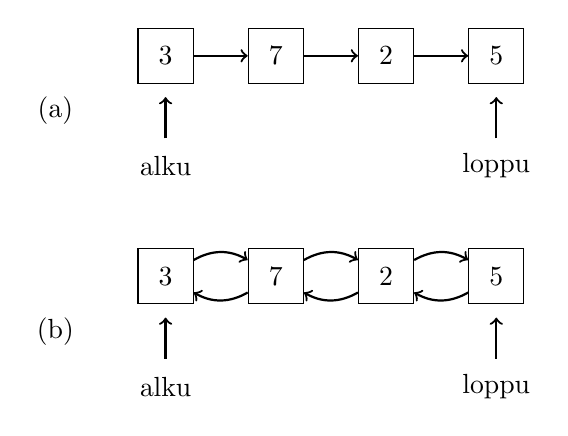
\begin{tikzpicture}[scale=0.7]
\begin{scope}
\node[draw, rectangle, minimum size=7mm] (1) at (0,0) {$3$};
\node[draw, rectangle, minimum size=7mm] (2) at (2,0) {$7$};
\node[draw, rectangle, minimum size=7mm] (3) at (4,0) {$2$};
\node[draw, rectangle, minimum size=7mm] (4) at (6,0) {$5$};
\path[draw,thick,->] (1) -- (2);
\path[draw,thick,->] (2) -- (3);
\path[draw,thick,->] (3) -- (4);
\node at (0,-2) {alku};
\node at (6,-2) {loppu};
\path[draw,thick,->] (0,-1.5) -- (0,-0.75);
\path[draw,thick,->] (6,-1.5) -- (6,-0.75);
\node at (-2,-1) {(a)};
\end{scope}
\begin{scope}[yshift=-4cm]
\node[draw, rectangle, minimum size=7mm] (1) at (0,0) {$3$};
\node[draw, rectangle, minimum size=7mm] (2) at (2,0) {$7$};
\node[draw, rectangle, minimum size=7mm] (3) at (4,0) {$2$};
\node[draw, rectangle, minimum size=7mm] (4) at (6,0) {$5$};
\path[draw,thick,->] (1) edge [bend left] (2);
\path[draw,thick,->] (2) edge [bend left] (3);
\path[draw,thick,->] (3) edge [bend left] (4);
\path[draw,thick,->] (4) edge [bend left] (3);
\path[draw,thick,->] (3) edge [bend left] (2);
\path[draw,thick,->] (2) edge [bend left] (1);
\node at (0,-2) {alku};
\node at (6,-2) {loppu};
\path[draw,thick,->] (0,-1.5) -- (0,-0.75);
\path[draw,thick,->] (6,-1.5) -- (6,-0.75);
\node at (-2,-1) {(b)};
\end{scope}
\end{tikzpicture}
\caption{Lista $[3,7,2,5]$ linkitettynä listana.
(a) Yhteen suuntaan linkitetty lista. (b) Kahteen suuntaan linkitetty lista.}
\label{fig:linlis}
\end{figure}

Kuva \ref{fig:linlis} näyttää esimerkkinä listan $[3,7,2,5]$
yhteen ja kahteen suuntaan linkitettynä.
Molemmissa listoissa tiedossamme on viittaukset listan
alkuun ja loppuun.
Yhteen suuntaan linkitetyssä listassa voimme käydä
läpi listan alkiot alusta loppuun,
kun taas kahteen suuntaan linkitetyssä listassa
voimme kulkea sekä alusta loppuun että lopusta alkuun.

Kaksisuuntainen linkitys on käytännössä järkevä tapa toteuttaa
linkitetty lista, ja oletamme jatkossa, että listamme on
kahteen suuntaan linkitetty ja meillä on tiedossa viittaukset
listan alkuun ja loppuun.

\subsection{Linkitetyt rakenteet}

Jokaisessa ohjelmointikielessä on omat keinonsa
linkitetyn rakenteen toteuttamiseen.
Javassa voimme toteuttaa linkitetyn rakenteen niin,
että jokainen solmu on oma olionsa.
Esimerkiksi voimme toteuttaa seuraavan luokan \texttt{Solmu},
jonka oliot toimivat linkitetyn listan solmuina:

\begin{code}
public class Solmu {
    public int arvo;
    public Solmu seuraava;
    public Solmu edellinen;

    public Solmu(int arvo, Solmu seuraava, Solmu edellinen) {
        this.arvo = arvo;
        this.seuraava = seuraava;
        this.edellinen = edellinen;
    }
}
\end{code}

Kenttä \texttt{arvo} kertoo solmun arvon,
kenttä \texttt{seuraava} osoittaa seuraavaan solmuun
ja kenttä \texttt{edellinen} osoittaa edelliseen solmuun.
Jos seuraavaa tai edellistä solmua ei ole,
viittauksen tilalla on arvo \texttt{null}.
Esimerkiksi seuraava koodi luo solmun,
jonka arvona on 5 ja joka ei viittaa mihinkään:

\begin{code}
Solmu s = new Solmu(5, null, null);
\end{code}

Seuraava koodi puolestaan näyttää, kuinka voimme luoda
tämän luokan avulla linkitetyn listan $[3,7,2,5]$:

\begin{code}
Solmu s1, s2, s3, s4;
s1 = new Solmu(3, s2, null);
s2 = new Solmu(7, s3, s1);
s3 = new Solmu(2, s4, s2);
s4 = new Solmu(5, null, s3);
\end{code}

Tämän jälkeen voisimme käydä listan läpi näin alusta loppuun:

\begin{code}
Solmu s = s1;
while (s != null) {
    System.out.println(s.arvo);
    s = s.seuraava;
}
\end{code}

Koodin tulostus on seuraava:

\begin{code}
3
7
2
5
\end{code}

\subsection{Listan operaatiot}

Linkitetyn listan etuna on,
että voimme lisätä ja poistaa
alkioita $O(1)$-ajassa kaikissa listan kohdissa.
Kun haluamme lisätä listalle alkion,
luomme ensin uuden solmun ja muutamme sitten
sen vieressä olevien solmujen viittauksia niin,
että ne viittaavat uuteen solmuun.
Vastaavasti kun haluamme poistaa alkion,
muutamme viittauksia niin, että solmu ohitetaan.

\begin{figure}
\center
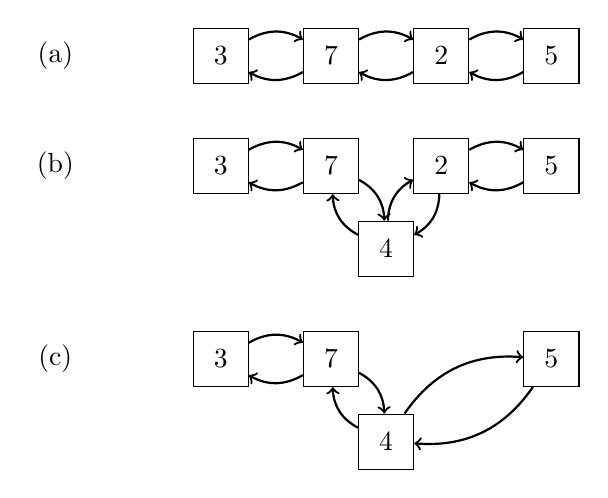
\begin{tikzpicture}[scale=0.7]
\begin{scope}
\node at (-3,0) {(a)};
\node[draw, rectangle, minimum size=7mm] (1) at (0,0) {$3$};
\node[draw, rectangle, minimum size=7mm] (2) at (2,0) {$7$};
\node[draw, rectangle, minimum size=7mm] (3) at (4,0) {$2$};
\node[draw, rectangle, minimum size=7mm] (4) at (6,0) {$5$};
\path[draw,thick,->] (1) edge [bend left] (2);
\path[draw,thick,->] (2) edge [bend left] (3);
\path[draw,thick,->] (3) edge [bend left] (4);
\path[draw,thick,->] (4) edge [bend left] (3);
\path[draw,thick,->] (3) edge [bend left] (2);
\path[draw,thick,->] (2) edge [bend left] (1);
\end{scope}
\begin{scope}[yshift=-2cm]
\node at (-3,0) {(b)};
\node[draw, rectangle, minimum size=7mm] (1) at (0,0) {$3$};
\node[draw, rectangle, minimum size=7mm] (2) at (2,0) {$7$};
\node[draw, rectangle, minimum size=7mm] (3) at (4,0) {$2$};
\node[draw, rectangle, minimum size=7mm] (4) at (6,0) {$5$};
\node[draw, rectangle, minimum size=7mm] (5) at (3,-1.5) {$4$};
\path[draw,thick,->] (1) edge [bend left] (2);
\path[draw,thick,->] (2) edge [bend left] (5);
\path[draw,thick,->] (5) edge [bend left] (3);
\path[draw,thick,->] (3) edge [bend left] (4);
\path[draw,thick,->] (4) edge [bend left] (3);
\path[draw,thick,->] (3) edge [bend left] (5);
\path[draw,thick,->] (5) edge [bend left] (2);
\path[draw,thick,->] (2) edge [bend left] (1);
\end{scope}
\begin{scope}[yshift=-5.5cm]
\node at (-3,0) {(c)};
\node[draw, rectangle, minimum size=7mm] (1) at (0,0) {$3$};
\node[draw, rectangle, minimum size=7mm] (2) at (2,0) {$7$};
\node[draw, rectangle, minimum size=7mm] (4) at (6,0) {$5$};
\node[draw, rectangle, minimum size=7mm] (5) at (3,-1.5) {$4$};
\path[draw,thick,->] (1) edge [bend left] (2);
\path[draw,thick,->] (2) edge [bend left] (5);
\path[draw,thick,->] (5) edge [bend left] (4);
\path[draw,thick,->] (4) edge [bend left] (5);
\path[draw,thick,->] (5) edge [bend left] (2);
\path[draw,thick,->] (2) edge [bend left] (1);
\end{scope}
\end{tikzpicture}
\caption{(a) Alkuperäinen lista $[3,7,2,5]$.
(b) Listan keskelle lisätään alkio $4$.
(c) Listasta poistetaan alkio $2$.}
\label{fig:lismuu}
\end{figure}

Kuva \ref{fig:lismuu} näyttää esimerkin linkitetyn listan käsittelystä.
Listan sisältönä on aluksi $[3,7,2,5]$.
Sitten lisämme listan keskelle alkion 4,
jolloin luomme ensin uuden solmun alkiolle ja muutamme
sitten viittauksia alkioiden 7 ja 2 välillä niin,
että alkio 4 tulee niiden väliin.
Lopuksi poistamme listasta alkion 2, jolloin yhdistämme
alkiot 4 ja 5 suoraan toisiinsa.

Pääsemme listan ensimmäiseen ja viimeiseen solmuun tehokkaasti,
koska meillä on muistissa viittaukset niihin.
Sen sijaan jos haluamme päästä johonkin muuhun listan kohtaan,
meidän täytyy aloittaa listan alusta tai lopusta ja kulkea askel
kerrallaan viittauksia seuraten.
Niinpä listan keskellä olevaan kohtaan pääseminen vie aikaa $O(n)$.
Joudumme liikkumaan solmuihin linkkejä pitkin, koska solmut voivat
olla eri puolilla muistia eikä meillä ole keinoa tietää suoraan,
mihin mikäkin solmu on tallennettu.

\subsection{Listojen vertailua}

\begin{table}
\center
\begin{tabular}{lrr}
operaatio & taulukkolista & linkitetty lista \\
\hline
pääsy listan alkuun & $O(1)$ & $O(1)$ \\
pääsy listan loppuun & $O(1)$ & $O(1)$ \\ 
pääsy listan keskelle &  $O(1)$ & $O(n)$ \\
lisäys/poisto listan alussa & $O(1)$ & $O(1)$ \\
lisäys/poisto listan lopussa & $O(1)$ & $O(1)$ \\ 
lisäys/poisto listan keskellä &  $O(n)$ & $O(1)$ \\
\end{tabular}
\caption{Taulukkolistan ja linkitetyn listan operaatioiden
aikavaativuuksia.}
\label{tab:taulin}
\end{table}

Taulukko \ref{tab:taulin} esittää yhteenvedon taulukkolistan ja
linkitetyn listan ominaisuuksista.
Kummassakin toteutuksessa on yksi operaatio,
joka ei ole tehokas.
Taulukkolistassa pääsemme tehokkaasti mihin tahansa listan
kohtaan, mutta on hidasta muokata listaa keskeltä.
Linkitetyssä listassa voimme muokata listaa mistä tahansa,
mutta keskelle pääseminen on hidasta.

Huomaa, että keskelle pääsemisen hitaus rajoittaa melko paljon
linkitetyn listan käyttämistä.
Vaikka pystymme sinänsä muokkaamaan listaa mistä tahansa kohdasta
tehokkaasti, meidän tulee ensin \emph{päästä} kyseiseen kohtaan.
Jos meillä on jostain syystä etukäteen tiedossa viittaus listan keskelle,
voimme muokata kyseistä kohtaa tehokkaasti,
mutta muuten meidän tulee ensin kulkea haluttuun kohtaan,
missä kuluu aikaa $O(n)$.

\section{Pino ja jono}

Listan avulla voimme toteuttaa myös kaksi erikoistunutta tietorakennetta,
pinon ja jonon, jotka sisältävät vain osan listan ominaisuuksista
eli niiden operaatiot ovat listaa rajoittuneempia.

\begin{figure}
\center
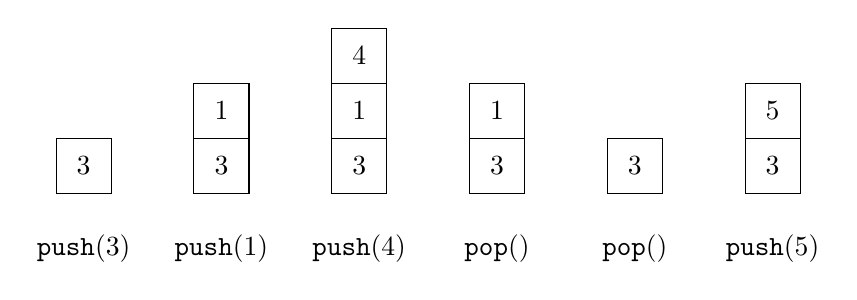
\begin{tikzpicture}[scale=0.7]
\begin{scope}[xshift=2.5cm]
\draw (0,0) grid (1,1);
\node at (0.5,0.5) {3};
\node at (0.5,-1) {$\texttt{push}(3)$};
\end{scope}
\begin{scope}[xshift=5cm]
\draw (0,0) grid (1,2);
\node at (0.5,0.5) {3};
\node at (0.5,1.5) {1};
\node at (0.5,-1) {$\texttt{push}(1)$};
\end{scope}
\begin{scope}[xshift=7.5cm]
\draw (0,0) grid (1,3);
\node at (0.5,0.5) {3};
\node at (0.5,1.5) {1};
\node at (0.5,2.5) {4};
\node at (0.5,-1) {$\texttt{push}(4)$};
\end{scope}
\begin{scope}[xshift=10cm]
\draw (0,0) grid (1,2);
\node at (0.5,0.5) {3};
\node at (0.5,1.5) {1};
\node at (0.5,-1) {$\texttt{pop}()$};
\end{scope}
\begin{scope}[xshift=12.5cm]
\draw (0,0) grid (1,1);
\node at (0.5,0.5) {3};
\node at (0.5,-1) {$\texttt{pop}()$};
\end{scope}
\begin{scope}[xshift=15cm]
\draw (0,0) grid (1,2);
\node at (0.5,0.5) {3};
\node at (0.5,1.5) {5};
\node at (0.5,-1) {$\texttt{push}(5)$};
\end{scope}
\end{tikzpicture}
\caption{Esimerkki pinon käsittelystä:
lisäämme tyhjään pinoon alkiot 3, 1 ja 4, poistamme kaksi ylintä
alkiota ja lisäämme lopuksi alkion 5.}
\label{fig:pinesi}
\end{figure}

\begin{figure}
\center
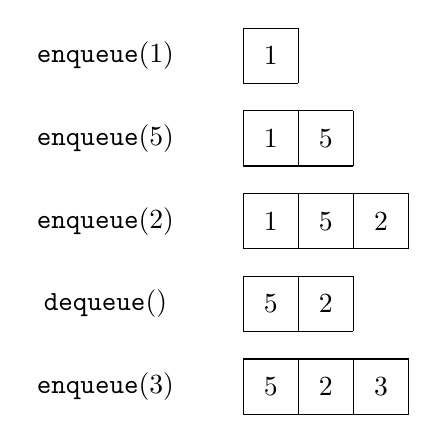
\begin{tikzpicture}[scale=0.7]
\begin{scope}
\draw (0,0) grid (1,1);
\node at (0.5,0.5) {$1$};
\node at (-2.5,0.5) {$\texttt{enqueue}(1)$};
\end{scope}
\begin{scope}[yshift=-1.5cm]
\draw (0,0) grid (2,1);
\node at (0.5,0.5) {$1$};
\node at (1.5,0.5) {$5$};
\node at (-2.5,0.5) {$\texttt{enqueue}(5)$};
\end{scope}
\begin{scope}[yshift=-3cm]
\draw (0,0) grid (3,1);
\node at (0.5,0.5) {$1$};
\node at (1.5,0.5) {$5$};
\node at (2.5,0.5) {$2$};
\node at (-2.5,0.5) {$\texttt{enqueue}(2)$};
\end{scope}
\begin{scope}[yshift=-4.5cm]
\draw (0,0) grid (2,1);
\node at (0.5,0.5) {$5$};
\node at (1.5,0.5) {$2$};
\node at (-2.5,0.5) {$\texttt{dequeue}()$};
\end{scope}
\begin{scope}[yshift=-6cm]
\draw (0,0) grid (3,1);
\node at (0.5,0.5) {$5$};
\node at (1.5,0.5) {$2$};
\node at (2.5,0.5) {$3$};
\node at (-2.5,0.5) {$\texttt{enqueue}(3)$};
\end{scope}
\end{tikzpicture}
\caption{Esimerkki jonon käsittelystä:
lisäämme tyhjään jonon alkiot 1, 5 ja 2,
poistamme yhden alkion ja lisäämme vielä alkion 3.}
\label{fig:jonesi}
\end{figure}

\index{pino}

\emph{Pino} (\emph{stack}) on tietorakenne,
jonka operaatiot ovat
alkion lisääminen pinon päälle (\texttt{push}),
ylimmän alkion poistaminen (\texttt{pop})
sekä ylimmän alkion hakeminen.
Esimerkiksi kuvassa \ref{fig:pinesi} lisäämme ensin tyhjään pinoon kolme alkiota,
poistamme sitten kaksi alkiota ja lisäämme vielä yhden alkion.

\index{jono}

\emph{Jono} (\emph{queue}) on tietorakenne, jossa voimme lisätä alkioita
jonon loppuun (\texttt{enqueue}),
poistaa alkioita jonon alusta (\texttt{dequeue})
ja hakea alkioita molemmista päistä.
Esimerkiksi kuvassa \ref{fig:jonesi} lisäämme ensin tyhjään jonoon
kolme alkiota, poistamme sitten yhden alkion ja lisämme vielä yhden alkion.

Pystymme toteuttamaan sekä pinon että jonon helposti
listana niin, että niiden operaatiot toimivat ajassa $O(1)$.
Mutta mitä järkeä on luoda uusia tietorakenteita,
jotka ovat \emph{huonompia} kuin lista?
Listassa voimme käsitellä mitä tahansa alkioita, mutta
pinossa ja jonossa emme pääse käsiksi keskellä oleviin alkioihin.
Selitys on siinä, että pino ja jono ovat hyödyllisiä 
\emph{käsit\-teitä} algoritmien suunnittelussa.
Voimme usein ajatella algoritmissa tarvittavaa
tietorakennetta pinona tai jonona ja toteuttaa sen sitten listana.

Tarkastellaan esimerkkinä tehtävää, jossa annettuna on
$n$ merkin pituinen \emph{sulkulauseke}, 
joka muodostuu kaarisulkeista \texttt{()} sekä
hakasulkeista \texttt{[]}.
Haluamme selvittää, onko lauseke \emph{oikein muodostettu} eli
onko jokaiselle aloittavalle sululle vastaava lopettava pari.
Esimerkiksi lauseke \texttt{[()]()} on oikein muodostettu,
kun taas lauseke \texttt{[()(])} ei ole.

Voimme ratkaista tehtävän $O(n)$-ajassa pinon avulla
käymällä läpi lausekkeen merkit vasemmalta oikealle.
Kun vastaan tulee aloittava sulku \texttt{(} tai \texttt{[},
lisäämme sen pinoon.
Kun taas vastaan tulee lopettava sulku \texttt{)} tai \texttt{]},
tutkimme, mikä on pinossa ylimpänä oleva merkki.
Jos merkki on vastaava aloittava sulku,
poistamme sen pinosta, ja muuten toteamme, että lauseke on virheellinen.
Jos lausekkeen läpikäynnin aikana ei esiinny virheitä
ja pino on lopuksi tyhjä, lauseke on oikein muodostettu.

\section{Javan toteutukset}

Javan standardikirjastossa on monia listojen toteutuksia,
jotka pohjautuvat taulukkolistaan tai linkitettyyn listaan.
Seuraavaksi tutustumme rakenteisiin, joista on usein
hyötyä algoritmien toteutuksessa.

\subsection{\texttt{ArrayList}-rakenne}

\texttt{ArrayList} on taulukkolista,
joka sallii tehokkaat lisäykset ja poistot listan lopussa.
Esimerkiksi seuraava koodi luo listan, lisää siihen alkiot
1, 2 ja 3 ja tulostaa listan sisällön.

\begin{code}
ArrayList<Integer> lista = new ArrayList<>();
lista.add(1);
lista.add(2);
lista.add(3);
System.out.println(lista); // [1, 2, 3]
\end{code}

Metodi \texttt{add} lisää oletuksena alkion listan loppuun
ja toimii siinä tapauksessa keskimäärin ajassa $O(1)$.

Koska lista on tallennettu taulukkona,
pääsemme myös tehokkaasti käsiksi sen alkioihin
kohdan perusteella.
Metodi \texttt{get} hakee tietyssä kohdassa olevan arvon,
ja metodi \texttt{set} muuttaa arvoa.
Esimerkiksi seuraava koodi tulostaa ensin
listan kohdassa 1 olevan alkion ja muuttaa sitten
sen arvoksi 5.

\begin{code}
System.out.println(lista.get(1)); // 2
lista.set(1,5);
System.out.println(lista.get(1)); // 5
\end{code}

Luokassa \texttt{Collections} on hyödyllisiä metodeita,
joiden avulla voimme muuttaa \texttt{ArrayList}-rakenteen
alkioiden järjestystä.
Seuraava esimerkkikoodi järjestää ensin listan,
muuttaa sitten sen järjestyksen käänteiseksi
ja sekoittaa lopuksi järjestyksen.

\begin{code}
Collections.sort(lista);
Collections.reverse(lista);
Collections.shuffle(lista);
\end{code}

\subsection{\texttt{ArrayDeque}-rakenne}

\texttt{ArrayDeque}-rakenne on taulukkolista,
joka sallii tehokkaat lisäykset ja poistot
sekä listan alussa että lopussa.
Alkioita voi lisätä
metodeilla \texttt{addFirst} ja \texttt{addLast}
ja poistaa
metodeilla \texttt{removeFirst} ja \texttt{removeLast}:

\begin{code}
ArrayDeque<Integer> lista = new ArrayDeque<>();
lista.addLast(1);
lista.addFirst(2);
lista.addLast(3);
System.out.println(lista); // [2, 1, 3]
lista.removeFirst();
System.out.println(lista); // [1, 3]
\end{code}

Lisäksi voimme hakea listan ensimmäisen ja viimeisen
alkion metodeilla \texttt{getFirst} ja \texttt{getLast}:

\begin{code}
ArrayDeque<Integer> lista = new ArrayDeque<>();
lista.addLast(1);
lista.addLast(2);
lista.addLast(3);
System.out.println(lista.getFirst()); // 1
System.out.println(lista.getLast()); // 3
\end{code}

Kaikki nämä metodit toimivat keskimäärin ajassa $O(1)$.
Rajoituksena on kuitenkin, että emme pääse käsiksi
listan keskellä oleviin alkioihin, vaan voimme käsitellä
vain listan alkua ja loppua.

\subsection{\texttt{LinkedList}-rakenne}

\texttt{LinkedList}-rakenne toteuttaa kaksisuuntaisen
linkitetyn listan, jossa voimme helposti lisätä ja poistaa
alkioita listan alussa ja lopussa.
Seuraava koodi esittelee asiaa:

\begin{code}
LinkedList<Integer> lista = new LinkedList<>();
lista.addLast(1);
lista.addFirst(2);
lista.addLast(3);
System.out.println(lista); // [2, 1, 3]
lista.removeFirst();
System.out.println(lista); // [1, 3]
\end{code}

\index{iteraattori}

Jos haluamme tehdä lisäyksiä ja poistoja muualla listassa,
meidän täytyy ottaa käyttöön \emph{iteraattori}, joka osoittaa haluttuun kohtaan.
Seuraava koodi luo iteraattorin, joka osoittaa ensin listan alkuun.
Sitten siirrämme iteraattoria kaksi askelta eteenpäin ja
lisäämme alkion 5 iteraattorin kohdalle eli listan
toisen ja kolmannen alkion väliin.

\begin{code}
ListIterator<Integer> x = lista.listIterator(0);
x.next();
x.next();
x.add(5);
\end{code}

\texttt{LinkedList} tarjoaa myös metodit
\texttt{get} ja \texttt{set}, joiden avulla
pääsemme käsiksi tietyssä kohdassa listalla olevaan alkioon.
Nämä metodit vievät kuitenkin aikaa $O(n)$,
koska joudumme kulkemaan ensin oikeaan kohtaan listan
alusta tai lopusta.
Tämän vuoksi \texttt{LinkedList} ei ole hyvä valinta,
jos haluamme käsitellä alkioita kohdan perusteella.

\section{Tehokkuusvertailu}

Tärkeä kysymys on, miten tehokkaita taulukkolista ja
linkitetty lista ovat \emph{käytännössä} ja kumpaa meidän
kannattaa käyttää, jos voimme valita.
Seuraavaksi vertailemme Javan taulukkolistan
(\texttt{ArrayList}) ja linkitetyn listan (\texttt{LinkedList})
käytännön tehokkuutta.

Testissä luomme ensin taulukon, joka sisältää luvut $1,2,\dots,n$
satunnaisessa järjestyksessä, sekä tyhjän listan.
Tämän jälkeen käymme taulukon läpi vasemmalta oikealle
ja lisäämme kunkin luvun listalle
sen oikealle paikalle niin, että lista säilyy järjestettynä.
Esimerkiksi jos listalla on ennestään alkiot $[2,3,6]$ ja seuraava
taulukon alkio on $4$, listasta tulee $[2,3,4,6]$.
Teemme saman testin taulukkolistalle ja linkitetylle listalle.

Taulukkolistan tapauksessa käymme listaa läpi alusta
muuttujalla $k$, kunnes tulemme kohtaan, johon uusi alkio kuuluu.
Tämän jälkeen lisäämme alkion kohtaan $k$ kutsumalla metodia \texttt{add}.

\begin{code}
for (int i = 0; i < n; i++) {
    int k = 0;
    while (k < lista.size() && lista.get(k) < taulu[i]) {
        k++;
    }
    lista.add(k,taulu[i]);
}
\end{code}

Linkitetyn listan tapauksessa luomme iteraattorin,
jonka avulla etsimme uuden alkion kohdan listan alusta lähtien.
Tämän jälkeen lisäämme alkion listalle iteraattorin osoittamaan kohtaan.

\begin{code}
for (int i = 0; i < n; i++) {
    ListIterator<Integer> x = lista.listIterator(0);
    while (x.hasNext()) {
        if (x.next() > taulu[i]) {
            x.previous();
            break;
        }
    }
    x.add(taulu[i]);
}
\end{code}

Taulukkolistassa sekä oikean kohdan etsiminen että alkion lisääminen
vievät aikaa $O(n)$, kun taas linkitetyssä listassa
oikean kohdan etsiminen vie aikaa $O(n)$, mutta alkion lisääminen
vie aikaa vain $O(1)$.
Mutta kuinka nopeasti koodit toimivat käytännössä?

\begin{table}
\center
\begin{tabular}{rrr}
parametri $n$ & \texttt{ArrayList} & \texttt{LinkedList} \\
\hline
$10000$ & 0.13 s & 0.38 s \\
$20000$ & 0.48 s & 1.20 s \\
$30000$ & 0.99 s & 2.70 s \\
$40000$ & 1.72 s & 5.15 s \\
$50000$ & 3.14 s & 8.99 s \\
\end{tabular}
\caption{Listarakenteiden tehokkuusvertailu.}
\label{tab:listes}
\end{table}

Taulukko \ref{tab:listes} näyttää testin tulokset.
Osoittautuu, että taulukkolista on selvästi
\emph{nopeampi} kuin linkitetty lista.
Näin käy siitä huolimatta, että taulukkolistassa
alkion lisääminen vie aikaa $O(n)$, mutta linkitetyssä
listassa aikaa kuluu $O(1)$.
Kysymys kuuluukin:

\subsubsection{Milloin kannattaa käyttää linkitettyä listaa?}

Tietorakenteiden maailmassa jokaiselle tietorakenteelle
on yleensä omat tietyt käyttötarkoituksensa,
joissa se erottuu edukseen muista tietorakenteista.
Linkitetty lista muodostaa kuitenkin poikkeuksen tähän sääntöön:
\emph{sitä ei kannata käyttää yleensä koskaan}.

\begin{figure}
\center
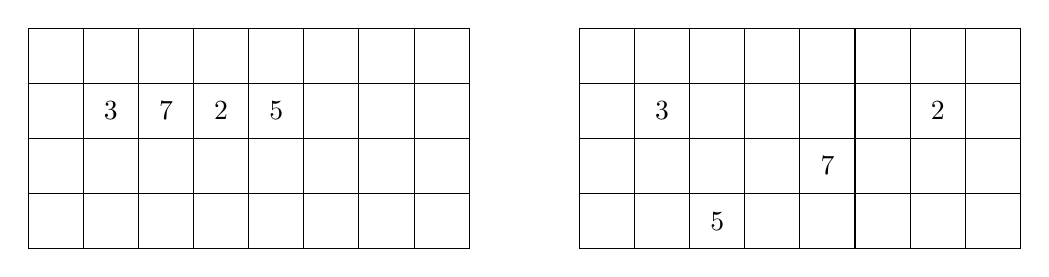
\begin{tikzpicture}[scale=0.7]
\begin{scope}
\draw (0,0) grid (8,4);
\node at (1.5,2.5) {3};
\node at (2.5,2.5) {7};
\node at (3.5,2.5) {2};
\node at (4.5,2.5) {5};
\end{scope}
\begin{scope}[xshift=10cm]
\draw (0,0) grid (8,4);
\node at (1.5,2.5) {3};
\node at (4.5,1.5) {7};
\node at (6.5,2.5) {2};
\node at (2.5,0.5) {5};
\end{scope}
\end{tikzpicture}
\caption{Taulukkolista ja linkitetty lista tietokoneen muistissa.}
\label{fig:taulin}
\end{figure}

Syynä tähän on, että nykyaikaiset tietokoneet
\emph{suosivat} taulukkolistan käyttämistä linkitetyn listan sijaan.
Kuvassa \ref{fig:taulin} näkyy, miten taulukkolista ja linkitetty lista
asettuvat tietokoneen muistissa.
Taulukkolistan alkiot ovat peräkkäin, kun taas linkitetyn
listan alkiot voivat olla eri puolilla muistia sekalaisessa
järjestyksessä.
Nykyaikaisen prosessorin välimuistit ja komentojen ennustus
on toteutettu niin, että ne ovat parhaimmillaan silloin,
kun tieto on tallennettu muistissa peräkkäin -- eli juuri kuten
taulukkolistassa.
Tämä näkyy käytännössä siinä, että taulukkolistan käsittely on selvästi
tehokkaampaa kuin linkitetyn listan käsittely.

Vaikka linkitetty lista ei ole käytännössä hyvä tietorakenne,
linkitetyn rakenteen idea on hyödyllinen
ja tarvitsemme sitä myöhemmin monimutkaisemmissa tietorakenteissa.
